\chapter{Using \LaTeX}\label{ch:usingLatex}

There are several reasons why one should prefer \LaTeX \space to a WYSIWYG word processor like Microsoft Word: \textsl{portability}, \textsl{lightness}, \textsl{security} are just a few of them (not to mention that \LaTeX \space is free). There is still a further reason that should definitely convince you to abandon MS Word for the development of a dissertation: you will never be able to produce professionally typeset and well-structured documents using most standard WYSIWYG tools.

\LaTeX \space is a free typesetting system that allows you to focus on content without bothering about the layout: the software takes care of the actual typesetting, structuring and page formatting, producing documents of astonishing elegance.

\section{Structure of this Template}

The file thesis.tex in the root of the directory (ThesisTemplate) is the main file of this template. This is the file that must be compiled to create the document. The thesis.tex document contains a lot of configuration settings. The only elements that require editing are details such as the title of the report, authors name and so forth. The only further addition to the file is to use the \emph{\textbackslash include} statement to include additional chapters into the report. One may also comment out the \emph{\textbackslash include} statements using the percentage sign (\%) to develop the report on a chapter by chapter basis. The BibTeX database thesis.bib is also included within the root. All the actual content of the report is divided up into directories each with a .tex file containing the chapter content.

\section{Using Figures}

 One can insert graphic elements using \LaTeX \space in a number of ways. Vector based imagery such as diagrams saved to the pdf format may use the \emph{\textbackslash includegraphics} command with the optional \emph{viewport} attribute to specify a precise area of the graphic to be included. Figures should also include a Caption and a Label for referencing.

When inserting a Figure (Figure~\ref{fig:using:MobilePhoneSuppliers2006MarketShare}) one uses the \emph{\textbackslash begin\{figure\}} and \emph{\textbackslash end\{figure\}} commands. The image presented is a vector graphic in the form of a pdf file. When working with such files it is usually necessary to include the optional \emph{viewport} attribute to designate the specific area in which to focus. The first pair of coordinates (x~\&~y) designate the pixel location of the lower left corner. The second pair identify the upper right hand corner. Modification of these coordinates allows one to focus in upon a particular area of interest within the vector image. The optional attribute [H] when beginning a Figure inserts the graphic element at the specified location. Other options such as [htb] (here, top, bottom) will place the graphic in the most suitable place that \LaTeX \space can find. This however can have a negative impact on memory allocation if a large number of images are to be found within the document.


\begin{figure}[H]
\centering
\includegraphics*[viewport= 80 130 725 505, width=.4\linewidth]{usingLatex/images/MobileMarketShare2006.pdf}
\caption{Mobile Phone Suppliers, Market Share 2006 (Millions of
Units Shipped)}
\label{fig:using:MobilePhoneSuppliers2006MarketShare}
\end{figure}

One may use the \emph{minipage} command when inserting two figures to span across the page. This allows for the subdividing of the page into a number of columns of specified width. Note the pie-charts presented here (Figure~\ref{fig:using:Example1} \&~\ref{fig:using:Example2}) are a bit small for viewing as printed matter. Zoom in on them using a pdf reader to see the advantage of printing diagrams (vector graphics) in pdf format.

\begin{figure}[H]
\begin{minipage}[t]{7.2cm}
\begin{center}
\includegraphics*[viewport= 80 130 725 505, width=.8\linewidth]{usingLatex/images/MobileMarketShare2006.pdf}
\caption{Caption for Figure}
\label{fig:using:Example1}
\end{center}
\end{minipage}
\hfill
\begin{minipage}[t]{7.2cm}
\begin{center}
\includegraphics*[viewport= 80 130 725 505, width=.8\linewidth]{usingLatex/images/MobileMarketShare2006.pdf}
\caption{Caption for Figure}
\label{fig:using:Example2}
\end{center}
\end{minipage}
\end{figure}

The example below (Figure~\ref{fig:using:samplepngImage}) demonstrates the insertion of a bitmap image. One can see that the extension for the image file isn't specified, as this template is setup to automatically search for .jpg, .png, .gif and .pdf images. The size of the displayed image within the document can be varied by adjusting the height and width attributes. To rotate an image 90 degrees an optional attribute can be added, for example [width=.4\textbackslash linewidth, angle=90].

\begin{figure}[H]
\begin{center}
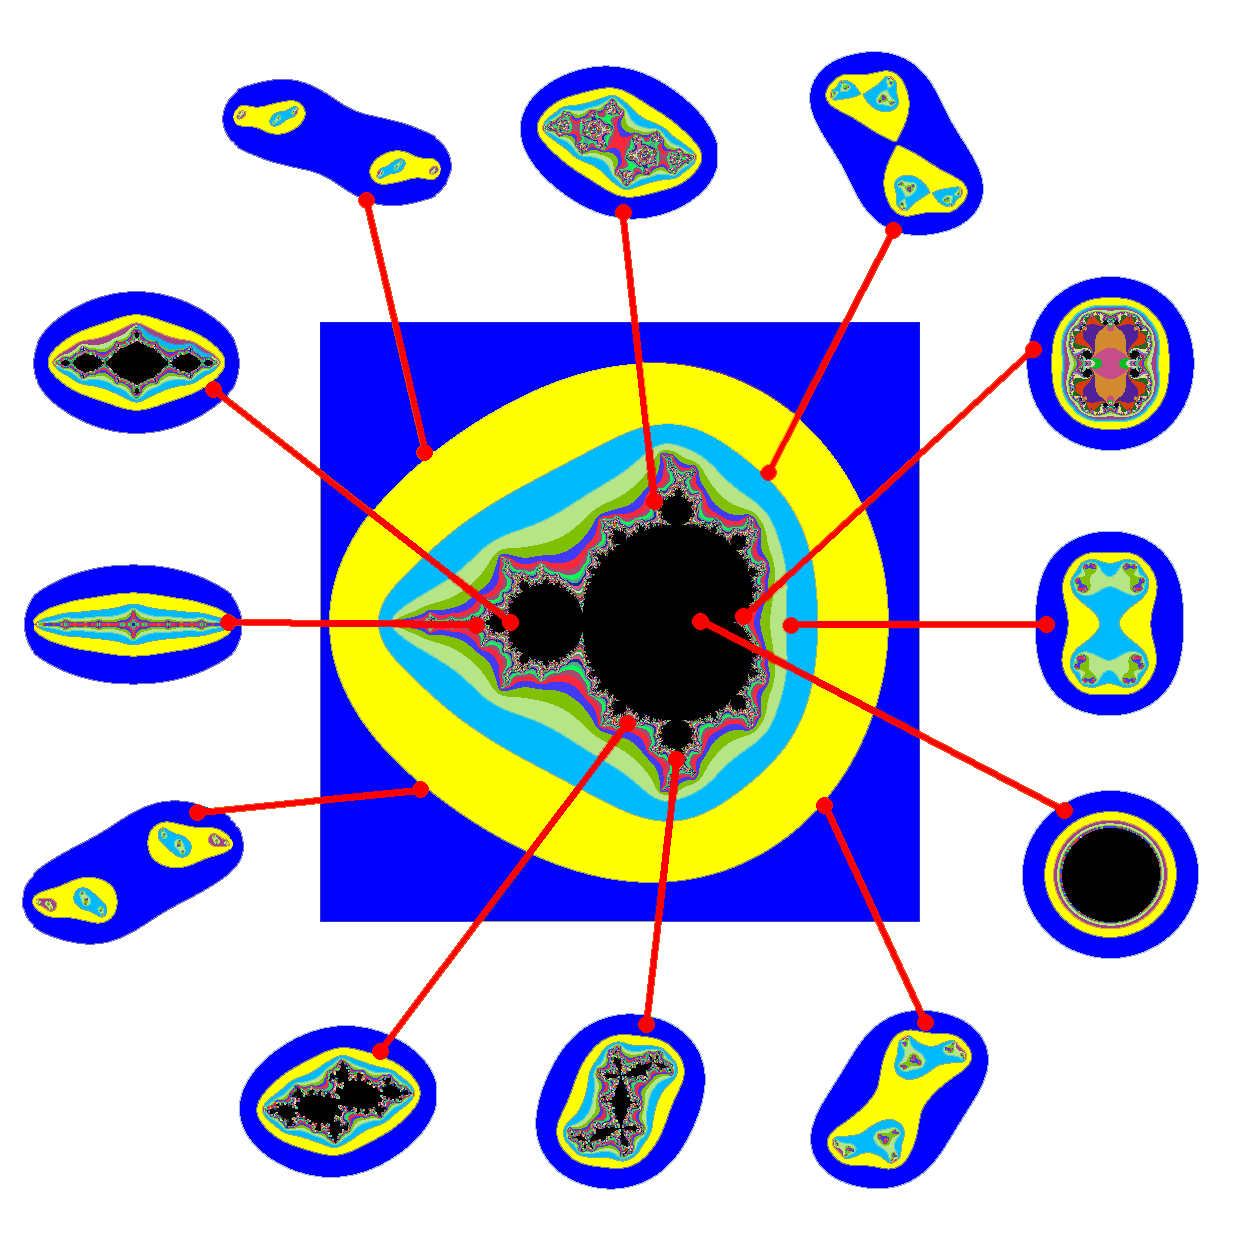
\includegraphics[width=.34\linewidth]{usingLatex/images/samplepng}
\caption{Caption for Bitmap Image Example} \label{fig:using:samplepngImage}
\end{center}
\end{figure}

\section{Referencing}

To refer to another part of the document one must use a combination of the \emph{\textbackslash ref} and \emph{\textbackslash label} commands. The label is a unique identifier, therefore when working with large documents it helps to give references meaningful names. Examples of this includes prefixing Table references with \emph{tab:}, figures with \emph{fig:}, chapters with \emph{ch:}. In very large documents in may also be useful to add an additional level of prefixing to represent the chapter the label is in. In this example chapter the tables and figures have the additional prefix of \emph{using} to represent the \emph{usingLatex} chapter. The tilde ($\sim$) is used to ensure that a reference remains as a single object. All instances of \emph{\textbackslash ref} should be preceded with the tilde.

\section{Citing Bibliographic References}

Bibliographic references are stored in a database (.bib file extension), this contains a list of articles, proceedings, books, thesis and so forth. Each type of publication has a number of required fields such as a unique identifier, author and title. To cite a references within the main body text one must use the \emph{\textbackslash cite} command as in the following examples. \cite{book:einsteinBrownianMovement} for example is well known for his work on Brownian Movement. The SETI@Home project \cite{web:berkeleyBOINC} is an example of a webpage citation. One can also work with articles \cite{art:Moller2003HWRastArch}, MSc Thesis \cite{msc:Edberg2007FluxgateMagnetometer}, PhD Thesis \cite{phd:Grace2004MiddlewareMobile} or articles within conference proceedings \cite{proc:Park2006UIMgtRmtRobots}. Several other types of article exist, but they are used to a lesser degree.

\subsection{The Harvard Bibliography Style}

The bibliographic references are laid out using the Harvard style. Further information about this style may be found at the following link (\url{https://library.rgu.ac.uk/RGUHarvard}). If you want parenthesis to enclose the reference, use \textit{parencite} instead of \textit{cite}. This would change the citation style in the previous paragraph to:

\parencite{book:einsteinBrownianMovement} for example is well known for his work on Brownian Movement.

\subsection{Compiling a BibTeX Database}

Having initially compiled the document using pdfLatex a number of helper files are created that aid in referencing and citations. One then must compile the bibtex database, followed by an additional two compiles using pdfLatex. Citing additional bibliographic references within the body of the document being produced will require the recompile of the bibtex database. In the case that the bibtex reference of a cited article cannot be found one will see a question mark [?] instead of the proper citation.

\subsection{The Harvard Bibliography Style}

The bibliographic references are laid out using the Harvard style. Further information about this style may be found at the following link (\url{https://library.rgu.ac.uk/RGUHarvard}). If you want parenthesis to enclose the reference, use \textit{parencite} instead of \textit{cite}.


\section{Working with Tables}

The data in a table (Table~\ref{tab:using:TableExample}) displays four columns of left-aligned data. The cell contents can be aligned to the left (l), right (r), or center (c). Vertical bars may sometimes be seen in tables but these generally look unprofessional. The Booktabs package \cite{web:Fear2005BookTabs} allows for the creation of professional looking tables as shown in the example.  The use of \emph{\textbackslash toprule}, \emph{\textbackslash midrule} and \emph{\textbackslash bottomrule} commands provided by the package allow for rules of varying thickness and spacing. Data elements (cells / columns) within a table are divided up using the ampersand (\&). To complete a row one must end with a double backslash (\textbackslash\textbackslash). Tables as with figures need a caption and a label.

\begin{table}[H]
\centering
\small
\begin{tabular}{llll}
\toprule \textbf{Heading 1}& \textbf{Heading 2}&\textbf{Heading 3}&\textbf{Heading 4}\\
\midrule
Cell A1 & Cell B2 & Cell C3 & Cell D4\\
Cell E1 & Cell F2 & Cell G3 & Cell H4\\
\bottomrule
\end{tabular}
\caption{Table Caption}\label{tab:using:TableExample}
\end{table}



One may find the following spreadsheet tool (\url{http://cobweb.ecn.purdue.edu/~zhang97/xls2latex/}) to be particularly useful for quickly converting tabular data in a spreadsheet to \LaTeX \space form. A complete list of instructions on how to use the tool are also present. The WinShell editor has an in-built GUI based utility to aid in the creation of the tabular data.

\section{Inserting an Algorithm}

The \emph{algorithm2e} environment may be used to generate algorithms (Algorithm~\ref{alg:using:SampleAlgorithm}). The following document (\url{http://www.tex.ac.uk/ctan/macros/latex/contrib/algorithm2e/algorithm2e.pdf}) provides detail of all the commands available within the package. If no algorithms are used within the document then comment out line 70 of the file {\tt thesis.tex} to remove the list of algorithms from the contents area.

\begin{algorithm}
%\dontprintsemicolon
\While{(RANK $<$ COMPSIZE)}{
    \If{(RANK == MASTER)}{
        generate random value \;
        \For{(each item K)}{
            get result \;
        }
    }
}
\caption{A Sample Algorithm} \label{alg:using:SampleAlgorithm}
\end{algorithm}

\section{Inserting Program Code Samples}

To insert small segments of program code (Listing~\ref{code:SampleCode}) that detail how interesting algorithms and so forth are implemented use the \emph{lstlisting} command. Inclusion of program code again requires a Caption and Label. Sample code from external files may also be included (Listing~\ref{code:externalSampleCodeLabel}), again one must supply a Caption and a Label as well as the relative path to the source file. Note a paragraph of text consisting of just a few lines is not a paragraph.

\break

\lstinputlisting[caption={The Caption for the Code Listing},label={code:externalSampleCodeLabel}]{usingLatex/myCodeFile.java}

\begin{lstlisting}[caption=Sample Program Code Listing, label=code:SampleCode]
if(rndVal==0){
    if(opType > 2){
       //do something
    }
}
\end{lstlisting}





\section{Working with Maths}
One can insert mathematical formula directly into a paragraph of text. The mathematical definition of the ``Cantor set'' is a good example of this in action
$\displaystyle\sum_{n=0}^\infty \frac{2^n}{3^{n+1}} = \frac{1}{3} +
\frac{2}{9} + \frac{4}{27} + \frac{8}{81} + \cdots =
\frac{1}{3}\left(\frac{1}{1-\frac{2}{3}}\right) = 1$. The previous equation demonstrates the use of sigma, fractions, large brackets, power, and dots. The function that defines the MSet is a simpler example of math in use $Z_{n+1} =
Z_{n}^2 + C$. Matrix Multiplication is typically regarded as an $O(n^3)$
operation. One may use the \emph{equation} environment for more complex mathematical formula that should standout. One may take for example the product  $C$ of two matrices $A \in M_{n,m}(R)$ and $B \in
M_{m,p}(R)$ to be defined as

\begin{equation}
(A \times B)_{ij} = \sum_{k=0} ^{m-1} a_{ik}b_{kj},~
i=0,...,n-1,~j=0,...,p-1.
\end{equation}

The sizes of the matrices must satisfy $(n \times m)(m \times p) =
(n \times p)$. Matrix multiplication is an associative process
thereby $a\cdot(b \cdot c) = (a \cdot b) \cdot c$. Essentially to
find the value of a particular cell $C_{i,j}$ it is necessary to
multiply row $i$ of the matrix $A$ with column $j$ of matrix $B$
summing all the multiplications.


\section{Required Software}

The implementation of \LaTeX \hspace{2 pt} typically used is MikTeX (\url{http://miktex.org/}). It is best to install the complete MiKTeX  system. Initially a small installer application must be downloaded and executed. This in-turn downloads the most recent implementation of the MikTeX system. The complete system is circa 500MB in size. Run the installer again and select the directory of the downloaded package.

To allow one to work with postscript documents a system called Ghostscript in required (\url{http://pages.cs.wisc.edu/~ghost/}). To be able to view these documents download and install GhostView (\url{http://pages.cs.wisc.edu/~ghost/gsview/index.htm}). The last element that is necessary is an editor. TeXnicCenter is a free download available at (\url{http://sourceforge.net/projects/texniccenter/}). An alternative is WinEdt a shareware ASCII editor (\url{http://www.winedt.com/}). WinEdt can be freely used for a 30 day period, after which one will periodically receive reminders to register the product. To demonstrate the use of an enumerated list, the software should be installed in the order detailed below. One final option for Windows users is WinShell (\url{http://www.winshell.de/}). An advantage of WinShell is its in-built BibTeX GUI editor. It also features a useful Table Wizard.

\begin{enumerate}
  \item MikTeX
  \item Ghostscript
  \item Ghostview
  \item Editor
\end{enumerate}

\section{Working with Quotes}
To surround a piece of text with double quotes one must place two single quotes on either side of the text. The double quote on the left is created using two left quotes (\lq) this is located just above the \emph{tab} key on the keyboard. The right hand double quote is created using two right hand quotes via (\rq) located just above and to the left of the right shift key. A properly formatted quotation should look like ``This is a quotation''. Notice how the direction of the quotes are opposite to one another.

\section{Further Information}
The Not so Short Introduction to LaTeX (\url{http://tobi.oetiker.ch/lshort/lshort.pdf}) is one useful source of further information on how to work with this system.

\section{Conclusion}
A short conclusion providing a summary of the chapter.
